\documentclass[12pt]{article}
\usepackage{graphicx}
\usepackage{wrapfig}
\openup 1em

\title{Security Vulnerabilities in the Veterinary Science Building}
\date{2017-05-09}
\author{Richard Coleman\
        \and
        Nora Cook
        \and
        Nakhai Bradley Johnson
        }
\begin{document}
        \maketitle
        \newpage
\section{Introduction}
        The Alfred State veterinary science building is a few miles away from the 
        Alfred State College and is used by students in the veterinary field. The
        building is closed completely on weekends. On weekdays it is open and while
        normally there are students there, during finals week it is almost empty.

\section{Security}
        \subsection{Vulnerabilities}
        
        \begin{wrapfigure}{R}{0.3\textwidth}
        \centering
        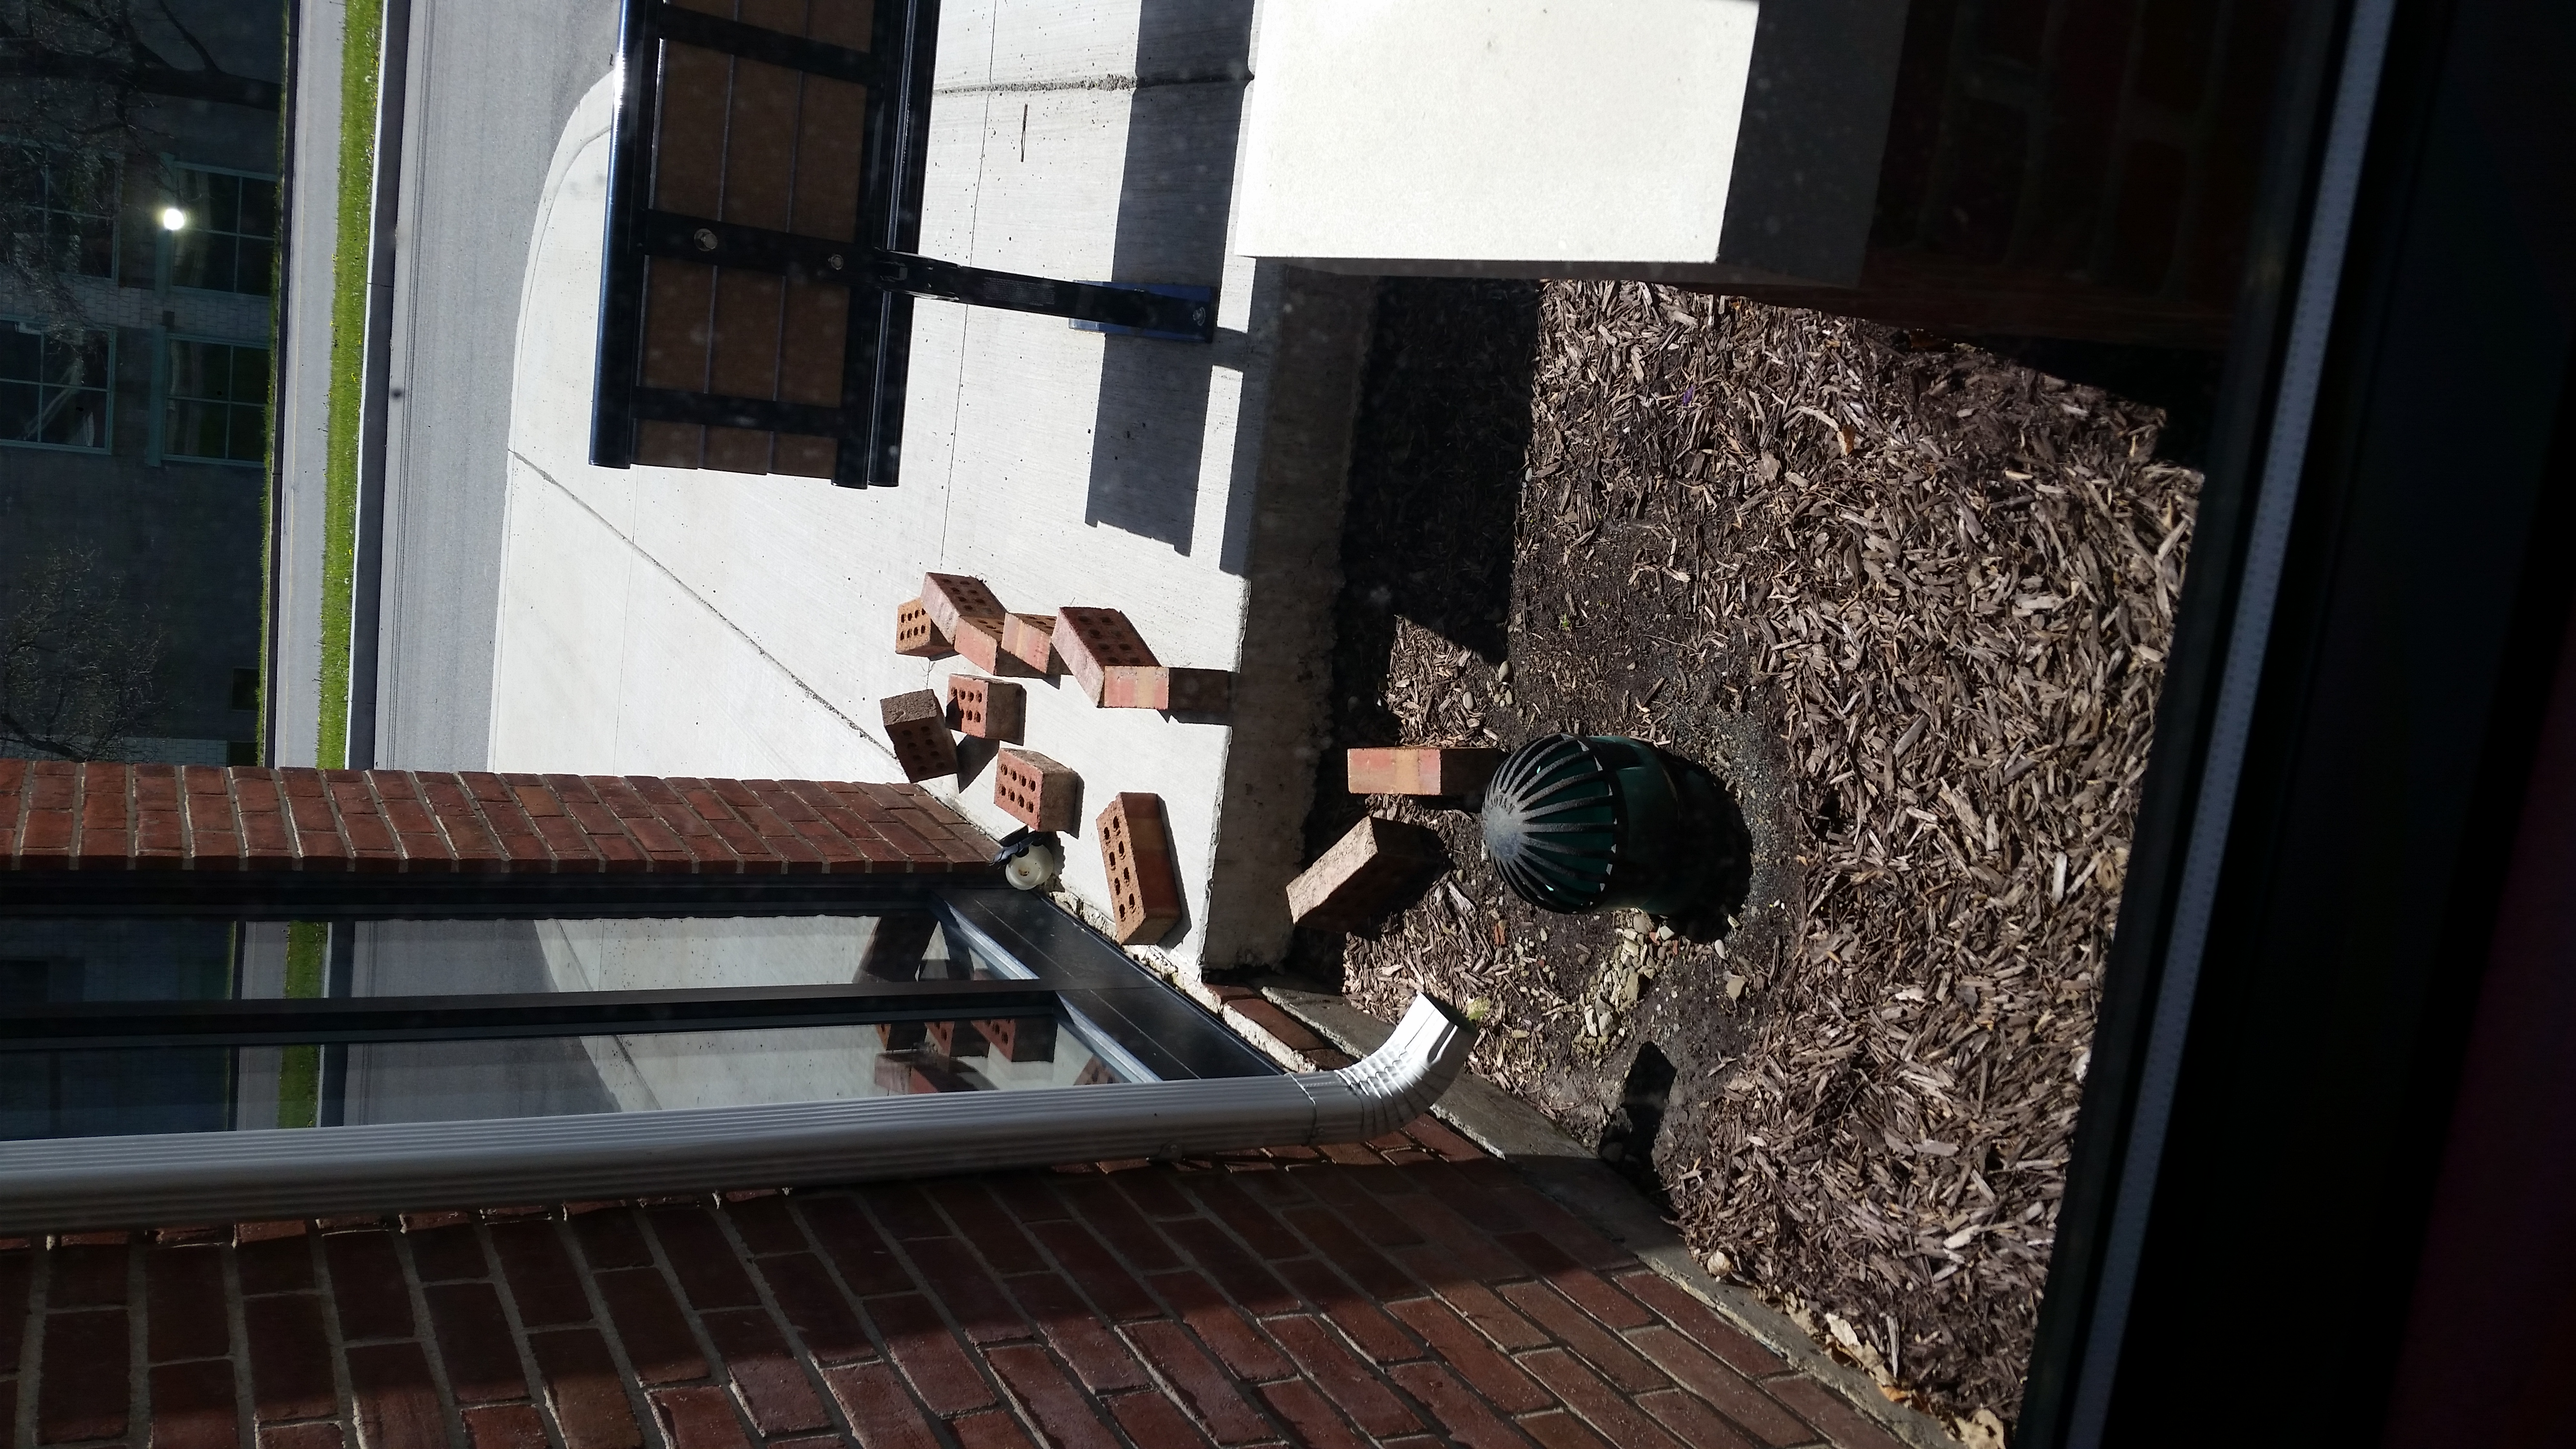
\includegraphics[width=0.5\textwidth, height=0.25\textwidth, angle=270]{img/bricks.jpg}
        \end{wrapfigure}

        When approaching the building from the main entrance you can see a pile of 
        bricks laying right beside the door. Someone that is very intent on breaking
        into the building could simply use any of those bricks to break any of the 
        large glass windows around the building.
        
        \begin{wrapfigure}{L}{0.3\textwidth}
        \centering
        \includegraphics[width=0.5\textwidth, height=0.25\textwidth, angle=270]{img/camera.jpg}
        \end{wrapfigure}

        After entering the building you can see only one security camera, our team
        did not find any more. There is also a secretary desk with a completely 
        unlocked computer. There are also two snakes in easily movable terrariums.

        An unlocked door leads into the rest of the building. On the left there is 
        an unlocked door which leads into a medical room with various medical
        equipment laying around. On the right there is a pharmacy and a another room
        both locked with a keypad for the former and a card swipe for the latter.

        Further down the corridor it opens up into a hallway lined by lockers, all of
        which were not locked, except for one. Down the left of the hallway there was
        another door that was left ajar. Most doors were unlocked in the whole building.
        The only person we came across seemed to be a professor who took us saying we
        were here for a class without question. 

        \subsection{Improvement}
        The first thing the building can do to improve its security is to increase the
        amount of cameras around the building. Policies also need to be put in place
        to make sure people are closing and locking doors when leaving rooms. 

        Snakes should also not be left in a place where they can be stolen. Staff and
        faculty should also be more aware in situations of potential social
        engineering. 

        Students should also be required to have a lock for any locker they use. There
        should also be more security than a simple key lock on each door considering
        many rooms contain medical equipment.

\section{Overview}
        Overall the building is pretty secure. Getting in without unlocked doors would
        prove to be a hassle and would attract too much attention for little gain. 
        With the primary means of entrance having a camera it would also be easy to 
        catch anyone who did try anything illegal as they must go through those doors.

        So, again overall good security. Could be improved as any place can be but it 
        is well secured for its purpose.

\end{document}
